\section{VLSI layout}

The problem consists in embed a complete binary tree with $n$ leaves in a grid using a minimal area. 
\begin{figure}[H]
    \centering
    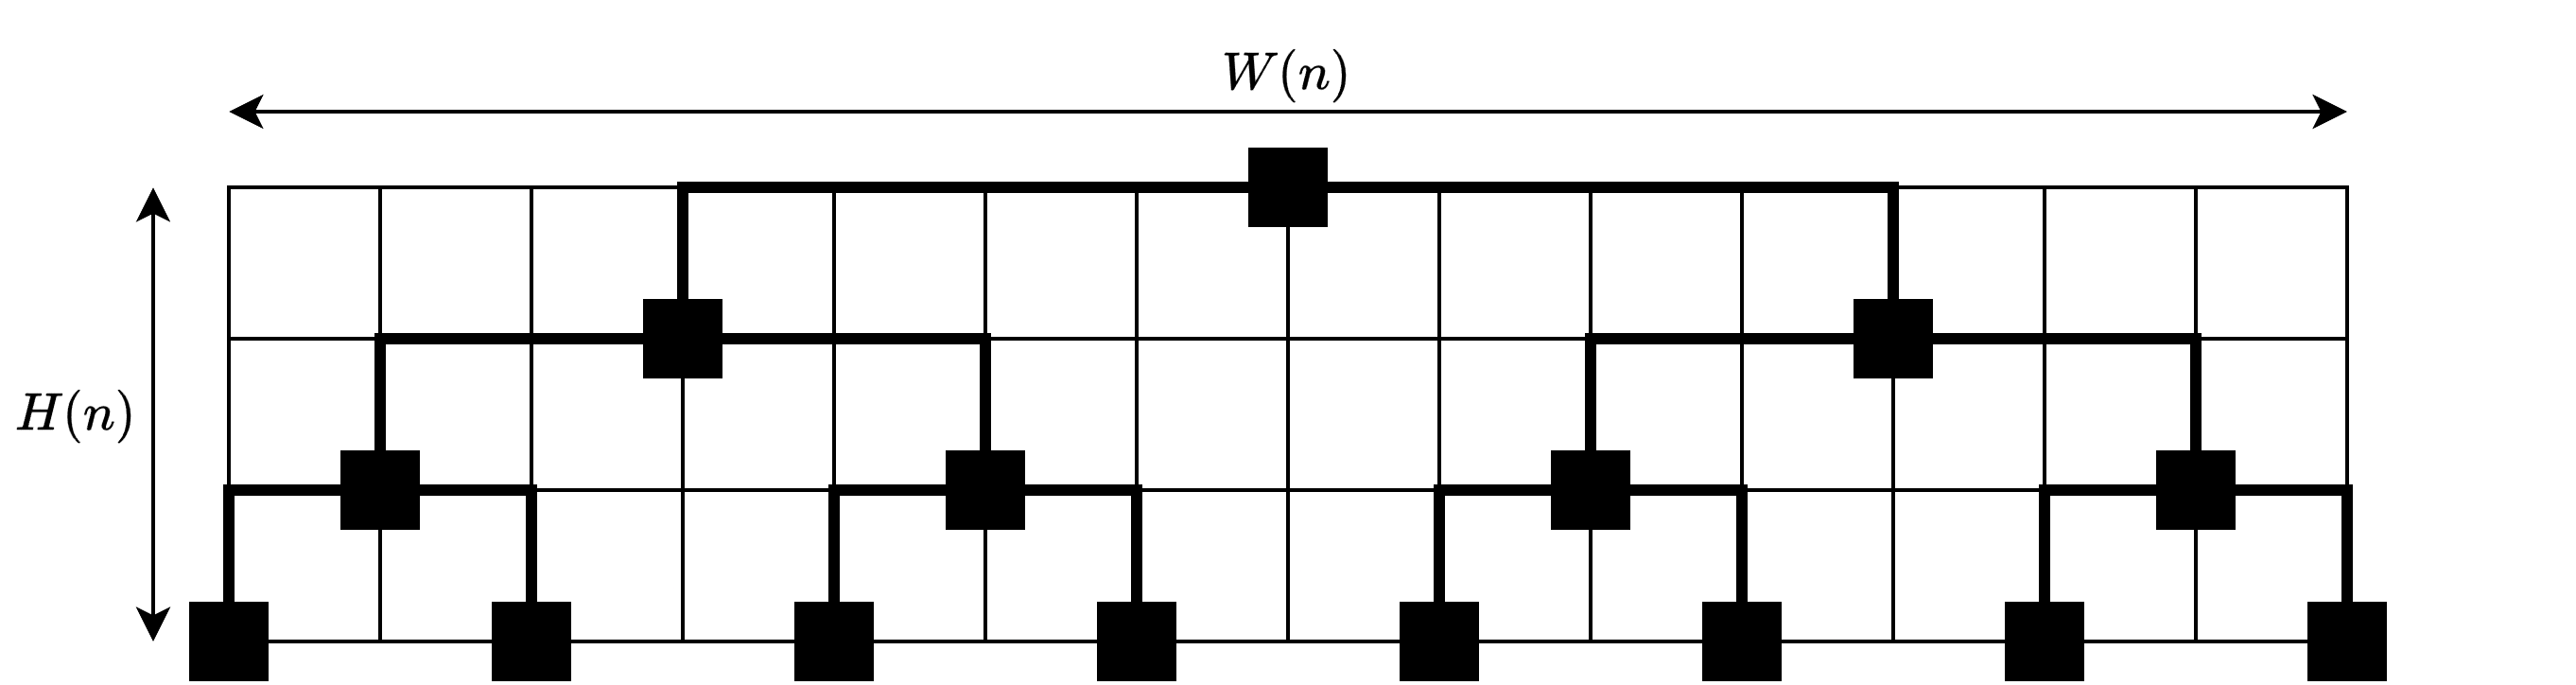
\includegraphics[width=0.75\linewidth]{images/vlsi.png}
    \caption{VLSI layout problem}
\end{figure}
Here, we have that the height of the tree is: 
\[H(n)=H\left(\dfrac{n}{2}\right)+\Theta(1)=\Theta(\log_2n)\]
Here, we have that the width of the tree is: 
\[W(n)=2W\left(\dfrac{n}{2}\right)+\Theta(1)=\Theta(n)\]
Thus, the total area of the grid is $\Theta(n\log_2n)$.

Another solution for this problem is to use an $h$-tree instead of a binary tree. 
\begin{figure}[H]
    \centering
    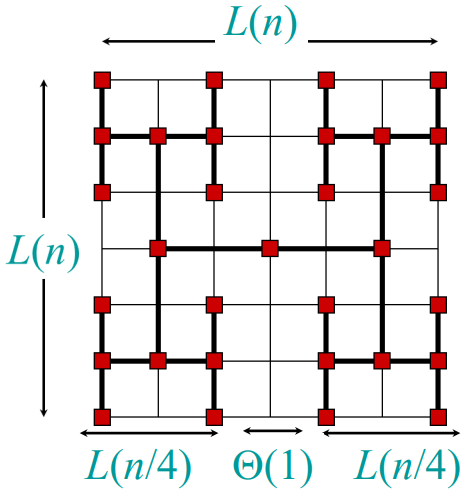
\includegraphics[width=0.5\linewidth]{images/vlsi1.png}
    \caption{VLSI layout problem}
\end{figure}
In this case we have that: 
\[L(n)=2L\left(\dfrac{n}{4}\right)+\Theta(1)=\Theta(\sqrt{n})\]
Thus, the total area is computed in $\Theta(n)$. 